\documentclass[11pt]{article}
\usepackage[utf8]{inputenc}
\usepackage[english]{babel}
\usepackage{amsmath}
\usepackage{graphicx}
\usepackage{float}
\usepackage{lipsum}
\usepackage{multicol}
\usepackage{xcolor}
\usepackage{tabularx}
\usepackage{booktabs}
\usepackage{hyperref}
\newcolumntype{Y}{>{\centering\arraybackslash}X}
\usepackage[left=2.00cm, right=2.00cm, top=2.00cm, bottom=2.00cm]{geometry}

\title{AN2DL Reports Template}

\begin{document}

\begin{figure}[H]
    \raggedright
    
\includegraphics[scale=0.4]{polimi.png} \hfill 
\includegraphics[scale=0.3]{airlab.jpeg}
\end{figure}

\vspace{5mm}

\begin{center}
    % Select between First and Second
    {\Large \textbf{AN2DL - First Homework Report}}\\
    \vspace{2mm}
    % Change with your Team Name
    {\Large \textbf{ANNamo bene}}\\
    \vspace{2mm}
    % Team Members Information
    {\large Michelangelo Stasi,}
    {\large Nicolò Tocalli,}
    {\large Elia Pontiggia}\\
    \vspace{2mm}
    % Codabench Nicknames
    {myke01,}
    {toky22,}
    {pontig}\\
    \vspace{2mm}
    % Matriculation Numbers
    {250299,}
    {247366,}
    {247274}\\
    \vspace{5mm}
    \today
\end{center}
\vspace{5mm}

\begin{multicols}{2}
    % \noindent \textit{Note: The following sections represent a suggested structure. Feel free to adapt them to better suit your specific project needs.}

    \section{Introduction}

    This project involves the implementation of a Convolutional Neural Network (CNN) for image classification. The CNN can be built entirely from scratch or include pre-trained layers provided by the Keras library.

    \section{Problem Analysis}

    The classification task in this project focuses on identifying different types of microscopic blood cells, such as basophils, neutrophils, and lymphocytes.

    \subsection{Dataset Description}

    The provided dataset contains nearly 14,000 RGB images of blood cells, categorized into 8 classes. Each image has a resolution of 96x96 pixels.

    \subsection{Data Preprocessing}

    During an initial inspection of the training set, we identified and removed 1,800 images containing outliers.
    Due to the limited number and variability of training images, we decided to augment the dataset by applying a range of random transformations. This approach aims to improve the generalization and robustness of our classifier.
    The transformations that, after parameter tuning, yielded the most significant improvements include the following:
    Random brightness, contrast, saturation and color degeneration to simulate real world variability. Rotations, translations, and flips to ensure invariance to orientation. Noise addition, cutout, and channel shuffle to enhance robustness against outliers.\\
    \noindent These transformations were implemented in two ways:
    \begin{itemize}
        \item \textbf{Off-line Augmentation:} Images were preprocessed to increase the dataset size by 2-3 times.
        \item \textbf{On-line Augmentation:} Transformations were applied during training to present the model with different versions of each image at every epoch.
    \end{itemize}
    Random zooms were excluded to avoid introducing bias, as cells from different classes might appear similar except for size. This could lead the model to classify images based on size rather than intrinsic features.\\
    Some of the pre-trained models we used already included preprocessing layers (e.g., normalization and resizing). In such cases, we adapted the preprocessing pipeline accordingly.\\
    We also observed a significant class imbalance in the dataset.~\ref{fig:dist}. To address this, we employed class weighting during training, which led to better performances than oversampling the minority classes.

    %\begin{figure}[H]
    %    \centering
    %    \includegraphics[width=0.50\linewidth]{classes.png}
    %    \caption{Distribution of the classes in the dataset}
    %    \label{fig:dist}
    %\end{figure}

    \section{Method}

    For this multi-class, single-label classification task, we utilized an 8-neuron Softmax output layer, with categorical cross-entropy as the loss function—a standard choice for such tasks.\\
    Our optimizer was Adam~\cite{Adam}, selected for its adaptive learning rate properties, after comparative tests revealed no substantial advantage in alternative optimizers like Lion.\\
    We incorporated dropout layers and early stopping to counteract overfitting. Given the limited dataset's size and variability, these techniques were critical in balancing model complexity with generalization capacity.

    \section{Experiments}

    \subsection{Baseline}

    We designed a basic CNN,  like the one presented during first lab session, to establish a performance baseline which highlighted the need for more sophisticated approaches due to its limited feature extraction capabilities.

    \subsection{State of the Art}

    We took inspiration from a novel lightweight multibranch CNN~\cite{Firat2024} including an inception module to improve accuracy with multi-scale convolutions, pyramid pooling module (PPM) to capture multi-scale context via feature pooling and depthwise squeeze-and-excitation block (DSEB) to  enable selective learning of relevant features. Despite the reported outstanding results in WBC classification, building it from scratch revealed poor generalization on the private Test-set, even after diverse augmentation and regularization techniques. This may be due to the lack of pre-trained weights for fine-tuning or differences in the training datasets, leading us to explore more robust architectures.

    \subsection{Transfer Learning and Fine tuning}

    Transitioning to pre-trained models like VGG16 and EfficientNet marked a significant improvement in performance. EfficientNet models, particularly EfficientNetV2M, were the most successful, so we mostly focused on them during the final stages of the project, given their strong balance between performance and cost-effectiveness.
    Regarding the set of layers to unfreeze during fine-tuning, we started by unfreezing only a few layers to maximize the benefits of the pre-trained model. We then gradually increased the number of unfrozen layers until we observed a decrease in performance, finally freezing 143 layers out of 719 for EfficientNetV2M.\\
    We decided to incrementally apply more aggressive augmentations, exploiting Augmix and Randaugment randomized pipelines. Then we achieved an impressive boost with CutMix and Mixup, powerful layers which should prevent the model from over-relying on single-instance features. In particular :
    \begin{itemize}
        \item \textbf{CutMix} helps the model to focus on multiple regions in the image, by "cutting and pasting" a patch from one image into another.
        \item \textbf{MixUp} interpolates two images and their labels, to create a blended image and corresponding soft label.
    \end{itemize}
    \begin{figure}[H]
        \centering
        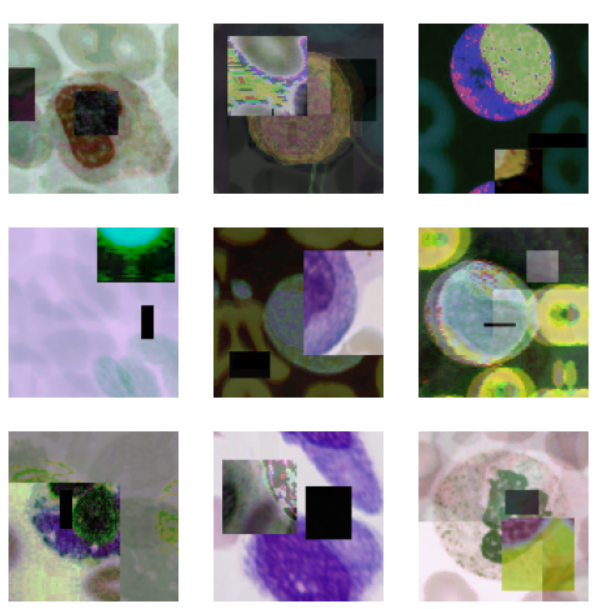
\includegraphics[width=0.50\linewidth]{augmented_sample.png}
        \caption{Samples from the final augmented dataset}
        \label{fig:noise}
    \end{figure}
    The models that achieved the best results are summarized in Table~\ref{tab:Performance}.\\
    \begin{table*}[t]
        \centering
        \setlength{\tabcolsep}{3pt}
        \caption{Performance of the models}
        \begin{tabularx}{\textwidth}{lYYYYYY}
            \toprule
            Model                     & Accuracy & Precision & Recall & F1     & Test 1 & Test 2 \\
            \midrule
            %Baseline w/o augmentation & 0.9297   & 0.9302    & 0.9297 & 0.9295 & 0.16   & -      \\
            Baseline w augmentation   & 0.8945   & 0.9025    & 0.8945 & 0.8957 & 0.19   & -      \\
            VGG16                     & 0.9498   & 0.9510    & 0.9498 & 0.9500 & 0.59   & -      \\
            EfficientnetV2S           & 0.9858   & 0.9859    & 0.9858 & 0.9858 & 0.92   & 0.94   \\
            EfficientnetV2M           & 0.9749   & 0.9750    & 0.9749 & 0.9748 & 0.90   & 0.95   \\
            EfficientNetV2L           & 0.9861   & 0.9862    & 0.9861 & 0.9861 & -      & 0.94   \\
            EfficientnetB2            & 0.9764   & 0.9679    & 0.9764 & 0.9674 & 0.77   & -      \\
            %Ensemble of V2S, B2, V2M  & 0.9941   & 0.9942    & 0.9941 & 0.9941 & 0.91   & -   \\
            \textbf{Ensemble of V2S, V2M, V2L}  & \textbf{0.9908}   & \textbf{0.9908}    & \textbf{0.9908} & \textbf{0.9908} & \textbf{-}   & \textbf{0.96}  \\
            Bagging of B2             & 0.8979   & 0.9078    & 0.8979 & 0.8980 & 0.71   & 0.72   \\
            \bottomrule
        \end{tabularx}
        \label{tab:Performance}
    \end{table*}
    Due to the computational intensity of training the models, we opted against k-fold cross-validation, despite it being ideal for the small dataset size. Instead, all local results were computed on a single validation set, comprising 20\% of the training set.\\
    Our models did not involve a large number of other hyperparameters to tune. The most significant ones were the learning rate and batch size, together with augmentation factors. We optimized these parameters through simple trial and error, occasionally integrating the \texttt{ReduceLROnPlateau} callback to  adaptively reduce learning rate when learning slowed down.

    \section{Discussion}

    Our models performed well on the validation set but showed slight overfitting, as indicated by worse results on Codabench compared to local machines. This was expected due to the absence of k-fold cross-validation. Nevertheless early stopping, dropout, robust data augmentation, tuning frozen layers, reducing batch size, and decreasing learning rate during fine tuning played a crucial role in mitigating overfitting.\\
    Models that generalized best to the test set often showed lower training accuracy due to aggressive augmentations, highlighting overfitting in earlier models.\\
    Trying an ensemble strategy, combining predictions from EfficientNetV2S, V2M, and V2L, revealed as the most robust approach to further increase accuracy. This method exploited the strengths of multiple configurations, smoothing over individual model weaknesses. While bagging could have further enhanced results, its computational cost made it unfeasible with the strong augmentations we used.\\
    The greatest breakthrough in model performance was achieved through the application of aggressive augmentations, particularly CutMix and Mixup layers, complemented with a 0.1 label smoothing to reduce overconfidence and help the model adapt to soft, interpolated labels.\\
    During the second phase we pushed our models to the limit by additionally increasing the magnitude of image transformations which explains the better performance of the models w.r.t. the first stage.

    \section{Conclusions}

    In this project, we implemented a Convolutional Neural Network for blood cell classification. This task presented several real-world challenges, such as a small and low-variability dataset, the presence of outliers, and a test set with a different distribution with respect to the training set.\\
    We addressed these challenges by augmenting the dataset with a variety of random transformations and removing problematic images.\\
    As one would do in a real-world scenario, we experimented with various pre-trained models and hyperparameters. Ultimately, the best performance on both phases was achieved through an ensemble averaging the predictions of EfficientNetV2S, EfficientNetB2, and EfficientNetB4 at first, and adding larger models like V2M and V2L in the last phase.\\
    We were glad to notice that our models were quite robust since the performance on the second test split was very similar to the first one when testing same architectures. This suggests that they were able to generalize well to unseen data and not overfit the first test split.
    
    \subsection*{Contributions}

    \textbf{Michelangelo:} Experiments with the VGG16 model and took care of the V2S EfficientNet model; in particular, implemented the augmentation layers inside these models' networks in addiction to the ones used in the pre-processing.\\
    \textbf{Nicolò:} Paper implementation, experiments with EfficientNet B2, V2M and V2L. Merge of the EfficientNet V2S with the implementation of Mixup and CutMix augmentation's layers. Ensemble of the best models obtained overall. \\
    \textbf{Elia:} Baseline creation with CNN from scratch, outliers removal, offline ligth augmentations, bagging of EfficientNetB2.\\
    
\end{multicols}
\newpage

% All the models created have an augmentation layer in the pre-processing phase, which has been personalized differently based on the performance of each model.
\bibliography{references}
\bibliographystyle{abbrv}
\end{document}
